% The very first thing in every latex file is the definition of the document class, in this case scrbook. There is also e.g. article, report, letter, beamer... The arguments in the square-brackets are optional arguments defining e.g. the font size (11pt) or the margins. bibliography=totoc ensures that the biblio appears in the table of contents (toc)
\documentclass[11pt,bibliography=totoc,openany,numbers=noendperiod]{scrbook}

% Import of packages and options regarding the whole document are outsourced in preamble.sty, which is a so-called style-file (that's why the -.sty ending). So similar to e.g. "import numpy" in Python, there is many packages which are loaded in there. So let's have a look at it...
\usepackage{preamble}
   

   
   
% Begin of the main body of your document. This command must be followed by an \end{document} command at the very end of the document.
\begin{document}
\mainmatter

% !!! Don't touch anything above here !!!
%-----------------------------------------------------------------------------------------------------------------
%-----------------------------------------------------------------------------------------------------------------
%-----------------------------------------------------------------------------------------------------------------



\section{CTD}
\label{app:ctd}

\textit{John Lennon \& Paul McCartney}

\vspace{1cm}

\lipsum[1]
\begin{figure}[htbp]		% typical way to include a figure. The option [htbp] means, that the compiler should try to place it Here first (that's why h first), then at the top of the next page (t as second letter), at the bottom of the page (b) and as last option wherever it fits best...
    \centering				% center the figure horizontally
    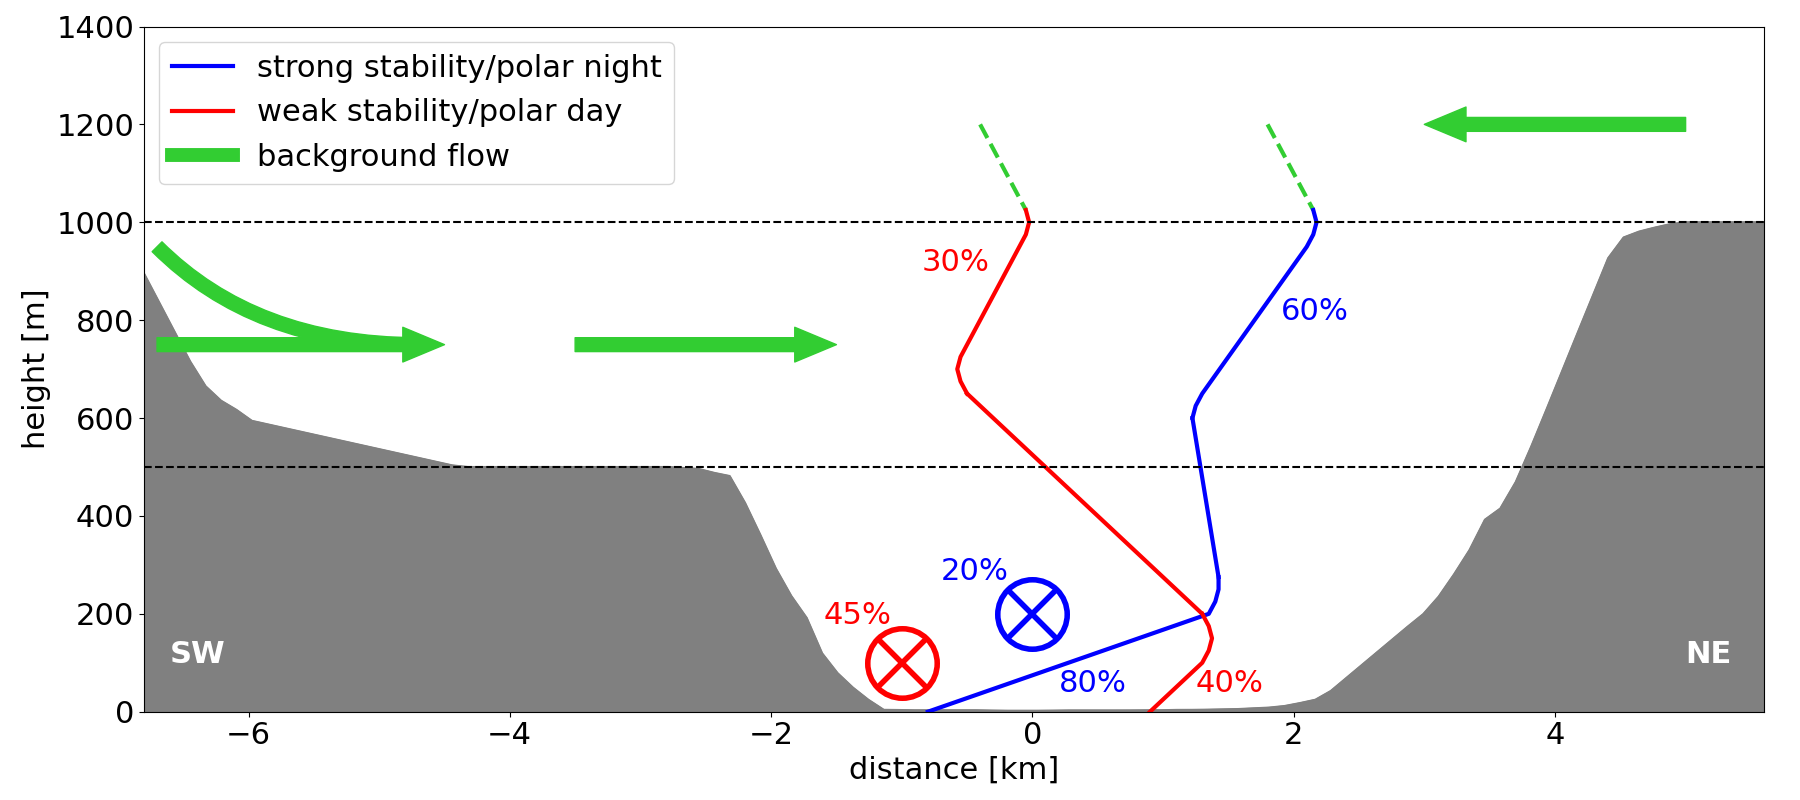
\includegraphics[width=\textwidth]{./figures_john/schematic_ABL.png}
    \vspace{-20pt}		% put the caption a little closer to the figure
    \caption[Short description for list of figures]{Longer description to be printed under the figure, can include references like \citep{stull1988introduction}} % The text in the curly brackets is what appears below the figure, the text in the square brackets appears in the list of figures. In that way, you can give it a shorter description for the list and a longer text to put actually with the figure.
	\label{app_john:fig1}		% label to reference to the figure in the text
\end{figure}


\bibliography{biblio_appendix_john}
\bibliographystyle{apalike}

%-----------------------------------------------------------------------------------------------------------------
%-----------------------------------------------------------------------------------------------------------------
%-----------------------------------------------------------------------------------------------------------------
   
\end{document}